\chapter{Diseño e implementación\label{05disenoTrabajo}}

El generador de datos se ha implementado en el lenguaje de programación Java debido a tres razones principales:

% TODO: Ver esto con Jesús mañana
\begin{enumerate}
  \item Entrada de los modelos Deimos: La compilación de los documentos de configuración de nuestro generador se realizan a través de una clase Xtext para. Esta compilación nos proporciona un gran valor añadido al crear un objeto Java con los tipos convertidos de los atributos del documento.
  % \item El lenguaje Java: Java, a pesar de ser un lenguaje algo antiguo (1995) es a día de hoy uno de los más usados. Según el ranking PYPL~\cite{pypl} Java es el segundo lenguaje de programación del pasado año 2021, y según la encuesta realizada por \href{StackOverflow}{www.StackOverflow.com} Java se mantiene como el 5 lenguaje más usado (FIgura \refname{figure:rankingLangs}) entre los más de 83000 programadores que realizaron su encuesta. Lo que nos asegura que el generador se implementa en un lenguaje vivo y que un gran porcentaje de programadores sabe y maneja a diario.

  % \begin{figure}[H]
  %   \centerline{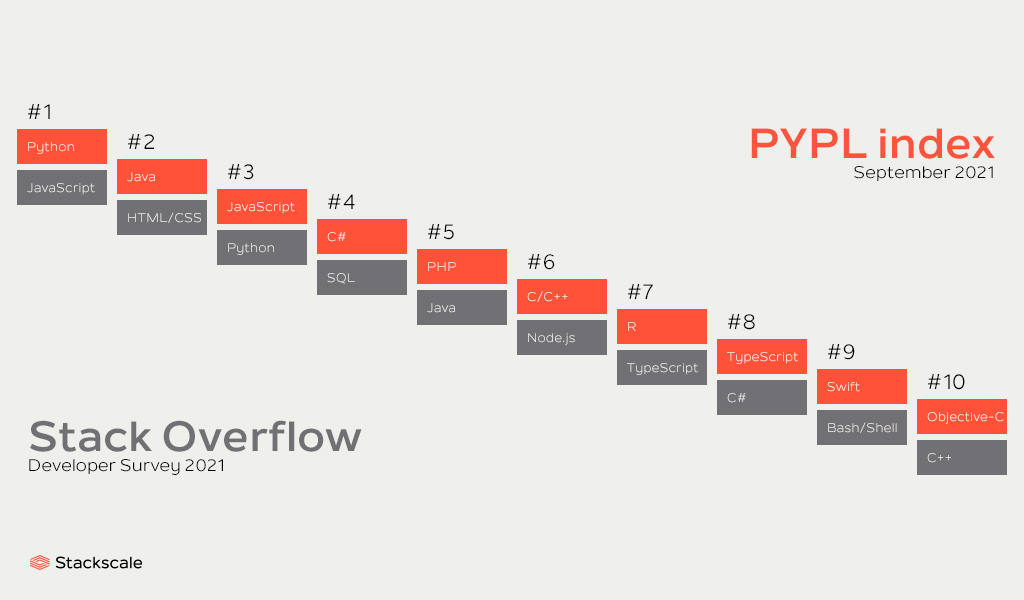
\includegraphics[width=1\textwidth]{rank_langs.jpg}}
  %   \caption{Ranking PYPL y StackOverflow lenguajes más populares/utilizados.}
  %   \label{figure:rankingLangs}
  % \end{figure}
  
  % \item Librerías y comunidad: Este experimentado lenguaje ofrece además una infinidad de librerías con años de desarrollo y una gran comunidad capaz de solucionar problemas lo que facilita el desarrollo del proyecto.
\end{enumerate}

Para organizar la estructura del proyecto se han utilizado los siguientes patrones de diseño:

\begin{itemize}
  \item Patrón fachada: Este patrón es utilizado a la hora de encapsular complejos proyecto que utilizan varios módulos de código haciéndolo sencillo. Nuestro generador provee una clase Generator que hace las veces de fachada para que el usuario solo tenga que molestarse en inicializar y ejecutar su método generate.
  \item Singleton: Los distintos servicios de input, output y rules han sido creados siguiendo el patrón Singleton para evitar la creación de dos servicios a partir del mismo fichero Deimos. Este patrón privatiza el constructor de un objeto a través de una función estática que comprueba si se ha creado ya una instancia y devolviendo ésta si ya existe.
  \item Composite: Este patrón ha sido utilizado a la hora de almacenar los distintos modificadores en cada una de las reglas. Consiste en crear una estructura de árbol donde el resultado de una operación es el mismo a la suma de sus operaciones hijas. De esta las reglas llaman a las operaciones de sus modificadores hijos.
  \item Memento: Tanto los outputs como los inputs guardan su estado para realizar las acciones correctas en cada momento, de esta manera los inputs pueden saber los datos que llevan leídos a la hora de escoger uno aleatoriamente y los outputs saben si la escritura que deben realizar es la última y por lo tanto deben cerrar el fichero o la conexión a la base de datos.
\end{itemize}



\section{Creación del generador}

El generador de datos posee una clase Generator que crea los servicios input, output y rules. Para ello es necesario crear una instancia de la clase Generator con dos atributos, el primero de ellos es una referencia al documento Deimos que podrá ser de tipo String referenciando la ruta donde se encuentra o un objeto File del mismo documento. El segundo parámetro deberá ser la clase del objeto que se quiere instanciar y del cual se genererarán entidades, esta clase debe cumplir los requisitos de una clase Bean de Java~\ref{09javaBean}. Para esto es importante conocer también el archivo Deimos, si se va a asociar una regla de tipo String con un atributo de la clase que no es de este tipo sucederá un error de conversión de tipo, igualmente sucede si la regla contiene un modificador strange que puede generar tipos extraños, el atributo al que vaya asociado deberá ser de tipo Object para que la conversión no de fallos. Por último se ha de tener en cuenta que si un atributo de la clase es un primitivo (por ejemplo int) y no su class wrap (Integer en este caso) si la regla devuelve un valor nulo no se devolverá null si no que se queda almacenado el valor por defecto de el tipo primitivo (en el caso de int es 0).

Una vez instanciada la clase, se puede llamar al método generate, el cual recibe de dos a cuatro parámetros. Los dos primero son obligatorios, primero un Objeto Map que asocia los atributos de la clase con reglas establecidas en el fichero Deimos, no es necesario crear una regla para cada atributo, si un atributo no se asocia con ninguna regla quedará sin instanciar en las entidades creadas. El siguiente atributo es el número de generaciones que el usuario desea realizar, los otros dos atributos son opcionales, la opción verbose indicará como transcurre la generación de las entidades con una barra de progreso, esta opción por defecto es false y no se recomienda utilizar si el usuario quiere mostrar por consola las entidades generadas ya que puede interferir en el proceso. Por último sizeWrite es un entero que obliga al generador a vaciar el pool de objetos generados por la salida cada cierto número de generaciones, por defecto su valor es mil y no se recomienda establecer un número muy alto para no sobrecargar la memoria del proceso.

\begin{lstlisting}[language=java]
package es.um.deimos.generator.example;

import java.io.IOException;
import java.util.HashMap;
import java.util.Map;
import es.um.deimos.generator.Generator;

public class Example1 {
  public static void main(String[] args) throws IOException {
    Generator<Persona> generator = new Generator<>("models/People.depr", Persona.class);

    Map<String, String> mapRules = new HashMap<String, String>() {
      private static final long serialVersionUID = 1L;
    {
      put("nombre","nameRule");
      put("altura","height");
      put("email","email");
      put("city","cityRule");
      put("provincia","provincia");
      put("numeroDeProvincia","nProvincia");
      put("yearBorn","yearBorn");
      put("fechaNacimiento","dateBorn");
      put("peso","weight");
      put("married","marriedRule");
      put("idPersona","idPersona");
      put("idPadre","anotherId");
    }};
    generator.generate(mapRules, 50000, true);
  }
}
\end{lstlisting}

En este ejemplo podemos comprobar la generación de 50000 datos para la siguiente clase llamada Persona donde utilizando el modelo `People.depr' donde se asignan reglas para cada uno de sus atributos.

Esta generación es posible gracias a el paquete java.lang.reflect el cual implementa métodos de ejecución de métodos Bean. El generador instancia un elemento en cada uno de las iteraciones realizadas (una por entidad creada) y modifica sus atributos a través de las funciones set de la clase con los valores devueltos por el servicio de reglas.

\subsection{Pseudoaleatoriedad de los datos}

La aleatoriedad a partir de semillas (seed) aportadas por el usuario era un aspecto clave en la generación de los datos. Para ello se ha utilizado la clase Random del paquete java.util.Random. Esta clase permite generar un objeto pseudoaleatorio proporcionando la seed que el usuario ha proporcionado, si esta no existiera, se utiliza el valor obtenido de la System.currentTimeMillis() que devuelve el número de milisegundos actuales desde el 1 de enero de 1970. El objeto Random creado es almacenado en el servicio Input, heredado a las clases inputs y además es utilizado por el servicio de reglas para que las generaciones de datos de las reglas que alberga sean igualmente pseudoaleatorias.

\section{Entrada de datos}

La entrada de datos del Generador se divide en una clase fabricante que encapsula el objeto de servicio, guardándolo de forma estática siguiendo el patrón Singleton. El servicio Input tiene como parámetro el objeto Deimos que representa el documento donde se encuentran los inputs establecidos y recorre todos estos filtrándolos por su tipo.

Todas las especificaciones heredan de la clase abstracta Input, con los siguientes atributos:

\begin{itemize}
  \item \textbf{inputName}: nombre adoptado por el usuario para el input.
  \item \textbf{inputSrc}: nombre del fichero o cadena de conexión.
  \item \textbf{random}: objeto aleatorio para la pseudoaleatoriedad del servicio.
  \item \textbf{order}: tipo de orden del input (sequential o random).
  \item \textbf{cycle}: tipo de ciclo (repeat o once).
\end{itemize}

Las clases que representan los tipos de inputs son las siguientes:

\begin{itemize}
  \item \textbf{InputJSON}: Utiliza la clase javax.json.Json de java para leer datos de un fichero en forma de array.

  \begin{lstlisting}[language=java]
    private void createInput() throws FileNotFoundException {
      arrayData = Json
          .createReader(new FileInputStream(new File(inputSrc)))
          .readArray();
    }
  \end{lstlisting}

  La clase carga un objeto de tipo JSONArray del paquete javax.json.JSONArray para ir leyendo en forma de streamReader sobre él.
  \item \textbf{InputCSV}: La clase InputCSV se ayuda de la librería jackson, esta librería es capaz tanto de leer ficheros CSV como de escribir objetos serializados en ellos. Por defecto carga fila a fila como un array de cadenas y va obteniendo la que el usuario le haya indicado.
  \item \textbf{InputPython}: Esta clase ejecuta a través del comando python el comando escrito en consola precedido del comando `python'. El resultado es obtenido en forma de streamReader y se considera un valor por línea. Una vez el stream ha llegado a su final y si el cycle del input se ha definido como repeat se volverá a ejecutar el comando.

  \emph{NOTA}: Si el programa de python utiliza algún mecanismo de aleatoriedad al proporcionar los datos esto ocasionaría romper con la pseudoaleatoriedad de la generación de los datos, por lo tanto, es recomendable que el ejecutable en python no contenga aleatoriedad o en su defecto que la misma pueda ser controlada por pseudoaleatoriedad al igual que nuestro generador.
  \item \textbf{InputTXT}: Los ficheros input son leídos linea a linea obteniendo una entrada de cada una de las mismas.
  \item \textbf{InputSQLQuery}: Esta clase utiliza la funcionalidad del paquete java.sql, el cual proporciona una API para abrir conexiones y realizar queries con distintos tipos de bases de datos relacionales a través de una cadena de conexión. El funcionamiento de esta clase es un híbrido de InputCSV e InputPython, por una parte recorre fila a fila obteniendo el dato de la columna seleccionada por el usuario y cuando las filas han finalizado y siempre que el input sea de ciclo repetitivo se volverá a abrir la conexión para realizar una nueva consulta.
  \begin{lstlisting}[language=java]
    Connection conn = null;
		Statement stat = null;
		try {
			conn = DriverManager.getConnection(this.stringConnection);
			stat = conn.createStatement();
			iteratorRows = stat.executeQuery(this.query);
    } catch(e) {
      //...
    }
  \end{lstlisting}
  \item \textbf{InputMongodbQuery}: Esta clase es semejante a la anterior con la diferencia que se apoya en el driver oficial de MongoDB para java `com.mongodb' para abrir conexiones y realizar consultas.
\end{itemize}

En cuanto a las opciones de ciclo y orden: Para los ciclos repetitivos reiniciamos la fuente de datos una vez estos se han acabado y seguimos devolviendo los datos, y en el caso de los de una generación devolvemos nulos o el dato por defecto. Para el caso de datos con ciclo aleatorio cargamos un numero variable de datos si la fuente devuelve estos uno a uno almacenándolos en una colección y seleccionando los datos a través del objeto random.

\section{Salida de datos}

El módulo de salida de datos contiene una clase servicio semejante a la de Input que se crea a través del modelo Deimos introducido y la clase de las entidades generadas, este módulo no necesita el seed de pseudo-generación debido a que las escrituras se realizarán en orden de entrada de la lista de objetos.

Debido a que el listado de objetos en memoria se debe ir vaciando para no provocar errores de espacio, el mismo se va escribiendo en la salida y borrando en la memoria, es por esto se ha definido un enumerado para conocer el estado de una escritura, esta puede ser de tres tipos `START', `CONTINUE' y `END'. Estos estados son necesarios a la hora de por ejemplo saber cuando abrir o cerrar una conexión a una base de a datos MongoDB o cuando escribir las cabeceras de un fichero CSV (se deben escribir en la primera línea).

Las clases creadas para la gestión de los Outputs heredan de una clase abstracta llamada Output la cual tiene dos funciones: writeDatas y close, la primera recibe una lista de objetos y el mencionado estado de la escritura, la función close tiene como finalidad cerrar las conexiones que pueda tener abierta la clase o hacer flush de los fichero de escritura, esta función puede ser llamada desde la función writeDatas cuando el estado de la escritura sea `END'. Las clases Outputs creadas son las siguientes:

\begin{itemize}
  \item \textbf{OutputConsole}: Escribe por consola la lista de objetos proporcionada utilizando el método toString de la misma, de esta forma se puede gestionar de forma sencilla el formato de salida de los atributos de las entidades.
  \item \textbf{OutputDatabase}: Utiliza el API de MongoDB de su driver Java para conectar a la conexión dada en el modelo Deimos y escribe los datos utilizando la función BulkWrite. Llama a la función close encargada de cerrar la conexión activa cuando la llamada a la función writeData contenga el parámetro estado END.
  \item \textbf{OutputFolder}: Alberga tres posible opciones `JSON', `CSV' y `TXT', en todas ellas crea o abre el fichero indicado en el modelo reemplazando su contenido existente y en cada una de las iteraciones escribe los datos obtenidos. Para el fichero TXT utiliza la función toString de la clase de la entidad al igual que sucedía en la salida por consola. CSV por su parte diferencia la primera escritura para escribir las cabeceras de la entidad. Por último, para que la salida por JSON no provocase un error a la hora de escribir varios elementos en el mismo archivo en varias escrituras distintas estos se escriben por separado escribiendo de manera manual las comas y los corchetes al inicio y final del documento para indicar el array generado.
  
  \begin{figure}[h!]
    \centerline{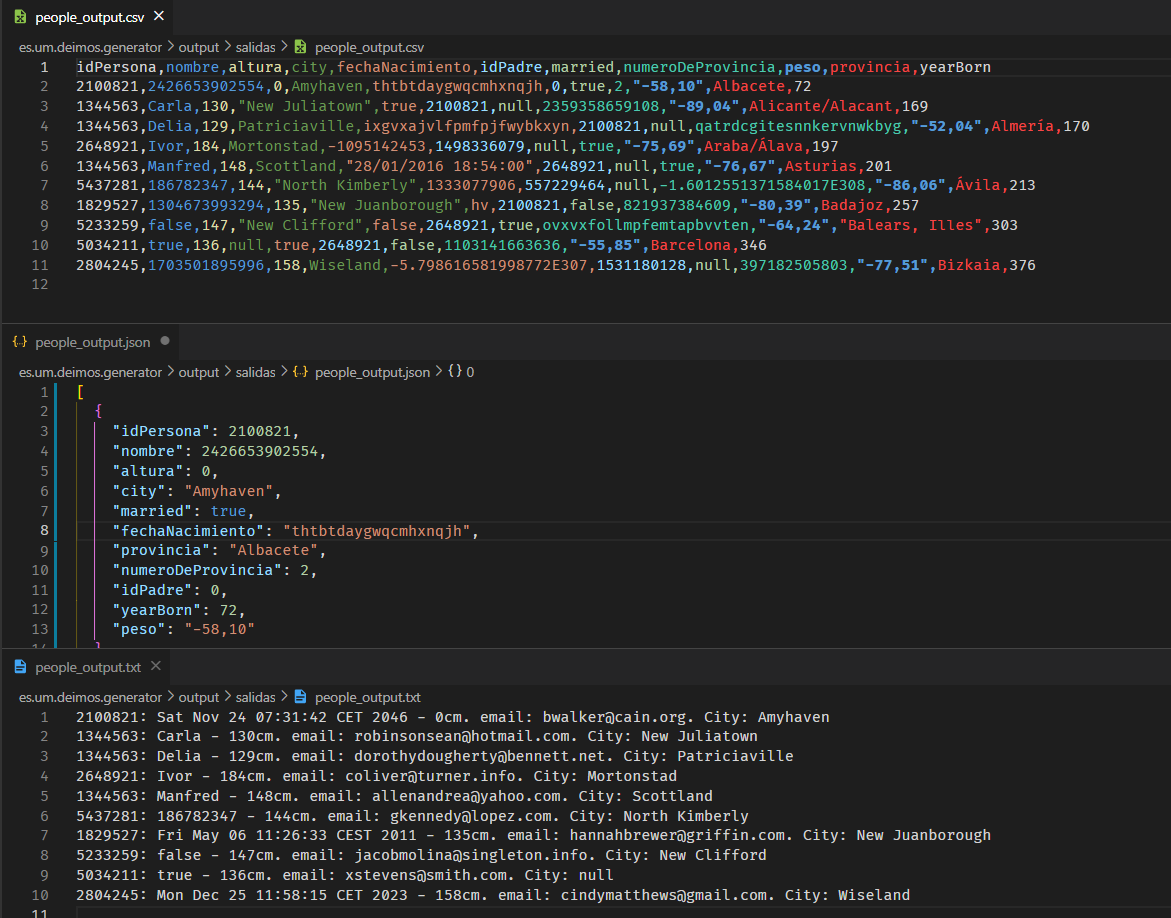
\includegraphics[width=1\textwidth]{ejemploOutputs.png}}
    \caption{Ejemplo de generación de datos y sus salidas.}
    \label{figure:outputExample}
  \end{figure}

  En la figura~\ref{figure:outputExample} podemos observar la misma salida para una generación de 10 entidades en los tres formatos de ficheros distintos.
\end{itemize}

\section{Reglas de datos}



%%% Local variables:
%%% TeX-master: "memoria.tex"
%%% coding: utf-8
%%% ispell-local-dictionary: "spanish"
%%% TeX-parse-self: t
%%% TeX-auto-save: t
%%% fill-column: 75
%%% End:

%  LocalWords:  NoSQL schemaless metadatos
